










\subsubsection*{Torsionspendel mit Hantel}
Hier wurde die Schwingungsdauer einer Hantel mit aufgelegten Scheiben beobachtet, wobei der Abstand $a$ des Scheibenschwerpunktes zur Rotationsachse variiert wurde. 



\begin{table}[h]
	\centering	
	\caption{Messdaten des Torsionspendels mit Hantel und aufgelegten Scheiben  }
	\begin{tabular}{|l|c|} 
		\hline 
		Messgröße	& Messwert  \\ 
		\hline 
		Länge des Drahtes $L_D$& \SI{1.8150\pm 0.0004 } {m} \\ 
		\hline 
		Masse der Achse $m_1$& \SI{0.21773}{kg} \\ 
		\hline 
		Radius der Achse $R_1$ & \SI{0.0599 \pm 0.0004}{m}  \\ 
		\hline 
		Länge der Achse $H_1$ &	\SI{0.27\pm 0.0004}	{\metre}	\\
		\hline
		Radius des Drahtes $R_D$ & \SI{2.50+-0.002 e-4} {m} \\ 
		\hline 
		Masse der aufgelegten Scheibe $m_2$& \SI{0.29728}{kg} \\ 
		\hline 
		Radius der aufgelegten Scheibe $R_2$ & \SI{0.0245 \pm 0.0004}{m}  \\ 
		\hline 
		Höhe der aufgelegten Scheibe $H_2$ &\SI{0.0204\pm0.00004 }{\metre}			\\
		\hline
	
	\end{tabular} 
	
	\label{tab:dataTH}
\end{table} 

Der Steinersche Satz sagt einen linearen Zusammenhang für \cref{fig:hantel} vorher, daher wurde eine Anpassung des Typs $T^2(2m_2 a^2)=b (2m a^2)+c$ gewählt, da der letzte Messpunkt deutlich Abseits einer gedachten Grade durch die anderen Messpunkte lag, wurde hier von einem groben Fehler ausgegangen und er wurde bei der Anpassung ausgelassen.


\begin{figure}[h]
	\centering
	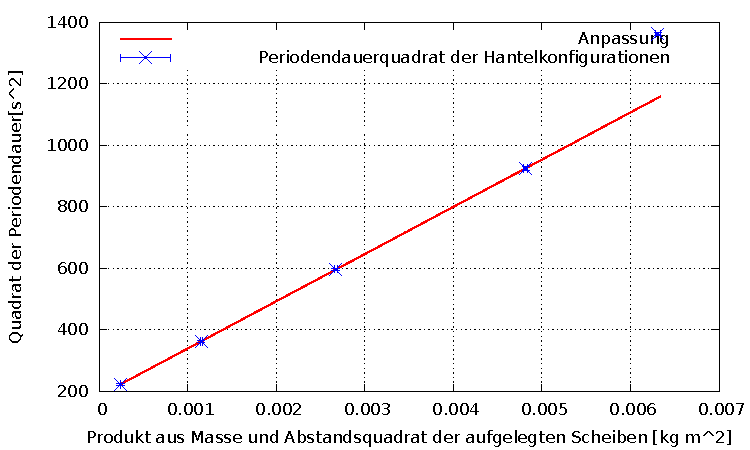
\includegraphics[width=0.7\linewidth]{auswertung/hantel/HantelF}
	\caption{Dargestellt werden die Messung mit Anpassung der Schwingungsdauern der Hantel mit aufgelegten Scheiben in verschiedenen Abständen zur Rotationsachse. Die Einheiten der Achsen sind so gewählt, dass die Messpunkte nach dem Steinerschen Satz linear sind.  }
	\label{fig:hantel}
\end{figure}

<<<<<<< HEAD
Der Steinersche Satz sagt einen linearen Zusammenhang für \cref{fig:hantel} vorher, daher wurde eine Anpassung des Typs $T^2(2m_2 a^2)=b (2m a^2)+c$ gewählt und man erhält nach der Anpassung\footnote{Die Anpassung wurde durch "Gnuplot" mit dem Levenberg–Marquardt Algorithmus vorgenommen.  } die Werte: $ b               = \SI{1.62   \pm 0.13 e+006}{\second \squared \per \kilogram \per \metre \squared} $ und $c               = \SI{ 1.3      +-0.5e3 }   {\second \squared}$. Aus der Steigung $b$ und Gleichung \ref{eq:hantelta} folgt durch Koeffzientenvergleich $D^*=\SI{2.4+-0.2e-5}{\kilogram \metre \squared \per \second \squared }$

%D^* exacter 0.0000243432



=======
Der Steinersche Satz sagt einen linearen Zusammenhang für \cref{fig:hantel} vorher, daher wurde eine Anpassung des Typs $T^2(2m_2 a^2)=b (2m a^2)+c$ gewählt, da der letzte Messpunkt deutlich Abseits einer gedachten Grade durch die anderen Messpunkte lag, wurde hier von einem groben Fehler ausgegangen und er wurde bei der Anpassung ausgelassen.
<<<<<<< HEAD
Man erhält nach der Anpassung\footnote{Die Anpassung wurde durch "Gnuplot" mit dem Levenberg–Marquardt Algorithmus vorgenommen.  } und unter Berücksichtigung des geringen Freiheitsgrades (2) die Werte:
 $ b               = \SI{1.5346 \pm 0.004 e+005}{\second \squared \per \kilogram \per \metre \squared} $ und $c               = \SI{186.587\pm 1.1}   {\second \squared}$. Aus der Steigung $b$ und Gleichung \ref{eq:hantelta} folgt durch Koeffzientenvergleich $D^*=\SI{8.19+-0.02e-5}{\kilogram \metre \squared \per \second \squared }$ Da jedoch der letzte Punkt so stark abweicht nehmen wir eine Unsicherheit von $\Delta D^*= \SI{\pm 2e-6}{\kilogram \metre \squared \per \second \squared }$ an.
=======
Man erhält nach der Anpassung\footnote{Die Anpassung wurde durch "Gnuplot" mit dem Levenberg–Marquardt Algorithmus vorgenommen.  } die Werte:
 $ b               = \SI{1.5346 \pm 0.003 e+005}{\second \squared \per \kilogram \per \metre \squared} $ und $c               = \SI{186.587\pm 0.8 }   {\second \squared}$. Aus der Steigung $b$ und Gleichung \ref{eq:hantelta} folgt durch Koeffzientenvergleich $D^*=\SI{8.189+-0.015e-5}{\kilogram \metre \squared \per \second \squared }$
>>>>>>> 7f87df1d78da537607abe4981a243fca98cd9d4b
>>>>>>> 0ca451c68b5b52fe32781abe016ca162189b079b


%t_p





Die Schwingungsdauer der Hantel ohne Scheiben $T_0$  betrug \SI{13.01 \pm 0.03}{s}. Es folgt mit Gleichung \ref{eq:hantelJ} für das Trägheitsmoment des Hantelstabes $J_1 = \SI{1.40+-0.04e-3}{\kilogram \metre \squared}$.



\begin{align}
	J=\frac{T^2 D^*}{4 \pi^2} \pm \frac{T^2 D^*}{4 \pi^2} \sqrt{
	\left(\frac{2 \Delta T}{T} \right)^2 + 	\left(\frac{\Delta D^*}{D^*} \right)^2 }
\label{eq:hantelJ}
\end{align}




Aus dem Parameter $c$ und der Gleichung \ref{eq:hantelta} und $a=0$  folgt für das Trägheitsmoment der Hantelscheiben mit Schwerpunkt auf der Rotationsachse die Gleichung \ref{eq:hantelJ2} und $J_2=\SI{5.1+-0.4e-5 }{\kilogram \metre \squared}$.


\begin{align}
		T^2&= \frac{4 \pi^2}{D^*}(J_1+2J_2+2m_2 a^2)
	\label{eq:hantelta}\\
J_2&=\frac{c D^*}{8 \pi ^2}-\frac{J_1}{2} \pm \sqrt{\left( \frac{c D^*}{8 \pi}\right) ^2\left( \left( \frac{\Delta c}{c}\right) ^2+  \left( \frac{\Delta D^*}{D^*}\right) ^2\right) + \left(\frac{J_1}{2}\right)^2 }\label{eq:hantelJ2}
\end{align}
\begin{align}
	J_{allg.}=\int r_{\perp}^2 \textrm{d}m
	\label{eq:Jallg}
\end{align}

Zum Vergleich wurden die theoretisch vorhergesagten Trägheitsmomente nach Gleichung \ref{eq:Jallg} bestimmt und in Tabelle \ref{tab:vglJ} mit den experimentell bestimmten zum Vergleich aufgeführt. 

\begin{table}[h!]
	\caption{Vergleich der experimentellen Trägheitsmomente mit den theoretisch berechneten}
	\begin{tabular}{|c|c|c|}
		\hline 
		Objekt &Theoretischer Wert	& Experimenteller Wert  \\ 
		\hline 
		Hantelstange $J_1$ &$\SI{1.324\pm 0.004 e-3}{}$	& $\SI{1.40\pm 0.04e-3}{}$ \\ 
		\hline 
		Scheibe $J_2$&  $\SI{5.76\pm 0.07e-5}{}$	&$\SI{5.1 \pm 0.5  e-04}{}$ \\ 
		\hline 
	\end{tabular} 
	\label{tab:vglJ}
\end{table}








\subsection{Diskussion}

%vgl mit lit wert am ehesten $\alpha$ Eisen $G=\SI{8.4 e9}{kg \per \metre \second \squared}$ abweichungen groß nicht aufgeführte legierung
Im Vergleich mit den Literaturwerten erscheint eine Stahllegierung wahrscheinlich. So besitzt zum Beispiel "CrV-Federstahl" oder "V2A-Stahl" ein Schubmodul\footnote{entnommen: Gerthsen Physik, Vogel 1977} $G=\SI{8.000 e10}{kg \per  \second \squared \metre}$.
Genauso Wahrscheinlich sind jedoch auch andere Stahllegierungen, da die Eigenschaften von den genauen Anteilen der Legierungsbestandteilen steuerbar sind und das gewünschte Schubmodul mit verschiedenen Zusätzen erreicht werden kann.\\
An den Werten in \cref{tab:vglJ}, dass der theoretische Wert für das Trägheitsmoment liegen jeweils in der $2 \sigma$-Umgebung des experimentell bestimmten Wertes und stellen somit keinen Widerspruch dar. Die weiteren berechneten Werte lassen sich nicht einordnen, da es sich um Materialkonstanten handelt und die Materialien nicht bekannt sind. Bei einer Weiterführung der Versuchsreihe wäre die Pendeldauer der Hantel für das größte $a$ zu wiederholen um zu überprüfen ob es sich wie angenommen um einen Fehler handelt oder ob die Abweichung reproduzierbar ist. Sollte eine höhere Genauigkeit erforderlich sein, sollte insbesondere $J_1$ genauer bestimmt werden, da dieser Wert für weitere Rechnungen benötigt wird. Eine höhere Genauigkeit von $D^*$, welches auch Grundlage weiterer Berechnungen ist, ist nur durch allgemeine Techniken wie mehr Abstände vermessen oder über viele Perioden mehrfach messen möglich und somit deutlich aufwendiger. 
%Tabbel Werte vgl Theorie exp....













